\documentclass[11pt]{article}
\usepackage[margin=1in]{geometry}
\usepackage{booktabs}
\usepackage{graphicx}
\usepackage{amsmath, amssymb}
\usepackage{xcolor}
\usepackage{hyperref}
\usepackage{caption}
\setlength{\parskip}{0.5\baselineskip}
\setlength{\parindent}{0pt}

\title{Cross-cultural recognition memory: intergroup correlation results}
\author{Bryan Medina --- generated by \texttt{make\_results\_report.py}}
\date{\today}

\begin{document}
\maketitle

\section*{Overview}
Intergroup itemwise correlations and paired-bootstrap comparisons for two conditions (\emph{Globalized-Music}, \emph{Industrial-Nature}) and two trial types (hits and false alarms). All numbers were produced by the Python pipeline in \texttt{Analysis-Scripts-v2/python/}; see \texttt{STATS.md} / \texttt{stats.pdf} for the methods. Bootstrap settings: $n_{\mathrm{boot}}=2000$ for pairwise CIs, $n_{\mathrm{boot}}=5000$ for the paired test, attenuation correction in \texttt{fixed} mode, participant-level resampling, \texttt{minResp}\,$=2$. Reported CIs are \textbf{percentile}: $\bigl[\mathrm{P}_{2.5}, \mathrm{P}_{97.5}\bigr]$ of the bootstrap distribution. Fisher-$z$ back-transformed and BCa alternatives are shown in the diagnostic table beneath each headline. BCa was considered as the headline (it is the textbook recommendation for skewed bootstraps) but misfires in cells with low within-group reliability --- for those cells the bias correction $\hat z_0$ is so large that $\hat r$ falls at or outside the BCa interval. The percentile CI is conservative under skew (wider than warranted) but doesn't break in that pathological way and is therefore the safer headline. The default $p$-value is the recentered-null variant.

\section*{Site partition and within-group reliabilities}
\begin{center}
\begin{tabular}{llccccc}
\toprule
Condition & Group & $n_{\mathrm{subj}}$ & $n_{\mathrm{items}}$ & $\hat{\rho}^{\mathrm{SB}}_{\mathrm{hit}}$ & $\hat{\rho}^{\mathrm{SB}}_{\mathrm{fa}}$ \\
\midrule
Globalized-Music & US & 96 & 80 & 0.776 & 0.865 \\
Globalized-Music & SanBorja & 63 & 80 & 0.716 & 0.741 \\
Globalized-Music & Tsimane & 68 & 80 & 0.217 & 0.695 \\
\midrule
Industrial-Nature & US & 141 & 80 & 0.782 & 0.910 \\
Industrial-Nature & SanBorja & 56 & 80 & 0.707 & 0.802 \\
Industrial-Nature & Tsimane & 81 & 80 & 0.707 & 0.804 \\
\midrule
NHS & US & 94 & 80 & 0.650 & 0.911 \\
NHS & SanBorja & 49 & 80 & 0.680 & 0.852 \\
NHS & Tsimane & 76 & 80 & 0.649 & 0.834 \\
\midrule
\bottomrule
\end{tabular}
\end{center}

\section*{Globalized-Music}

\subsubsection*{Hits}

\subsection*{Pairwise intergroup correlations (percentile 95\% CIs)}
\begin{center}
\begin{tabular}{lcccc}
\toprule
Pair & $\hat r$ (raw) & 95\% CI & $\hat r^*$ (corrected) & 95\% CI \\
\midrule
US$-$SB & +0.478 & [+0.223, +0.515] & +0.641 & [+0.299, +0.690] \\
US$-$Tsi & +0.426 & [+0.115, +0.429] & +1.038 & [+0.280, +1.045] \\
SB$-$Tsi & +0.413 & [+0.102, +0.459] & +1.047 & [+0.259, +1.163] \\
\bottomrule
\end{tabular}
\end{center}

\subsection*{Diagnostic --- alternative CIs on corrected $\hat r^*$}
\begin{center}
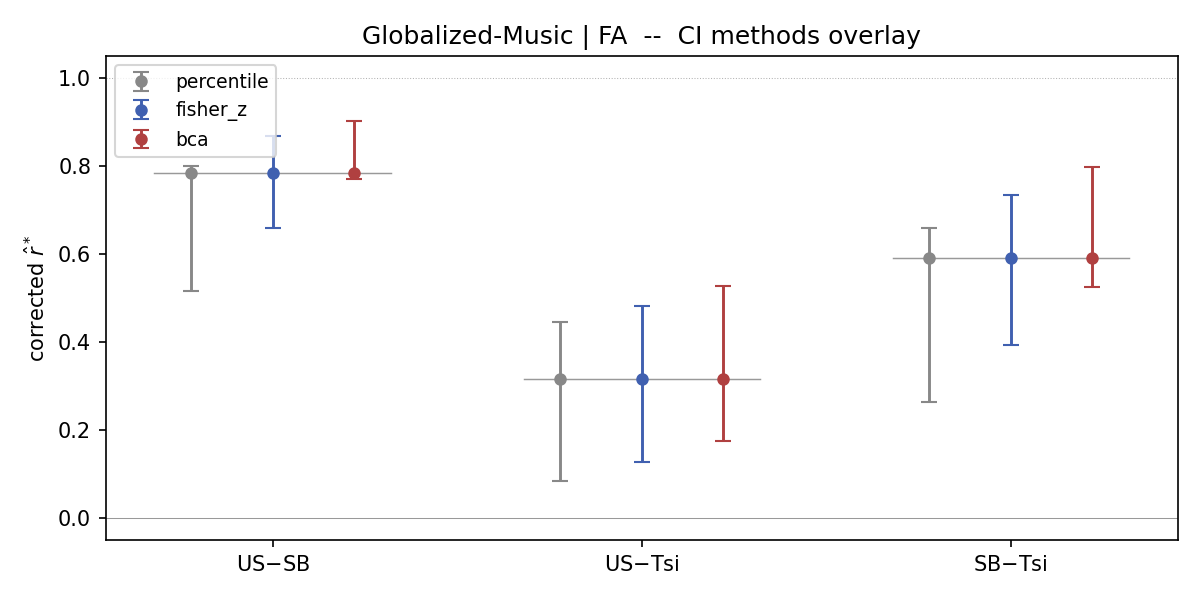
\includegraphics[width=0.85\textwidth]{figures/ci_compare_Globalized-Music_fa.png}
\end{center}

\begin{center}
\begin{tabular}{lcccc}
\toprule
Pair & $\hat r^*$ & Percentile 95\% CI & Fisher-$z$ 95\% CI & BCa 95\% CI \\
\midrule
US$-$SB & +0.641 & [+0.299, +0.690] & [+0.466, +0.768] & [+0.601, +0.793] \\
US$-$Tsi & +1.038 & [+0.280, +1.045] & [+1.000, +1.000] & [+1.031, +1.304] \\
SB$-$Tsi & +1.047 & [+0.259, +1.163] & [+0.998, +1.000] & [+0.919, +1.438] \\
\bottomrule
\end{tabular}
\end{center}

\subsection*{Stimulus-bootstrap diagnostic --- CIs on corrected $\hat r^*$ (resampling stimuli, not participants)}
\begin{center}
\begin{tabular}{lcccc}
\toprule
Pair & $\hat r^*$ & Percentile 95\% CI & Fisher-$z$ 95\% CI & BCa 95\% CI \\
\midrule
US$-$SB & +0.641 & [+0.371, +0.847] & [+0.307, +0.835] & [+0.369, +0.847] \\
US$-$Tsi & +1.038 & [+0.544, +1.435] & [+0.898, +1.000] & [+0.546, +1.436] \\
SB$-$Tsi & +1.047 & [+0.542, +1.468] & [+0.908, +1.000] & [+0.505, +1.455] \\
\bottomrule
\end{tabular}
\end{center}

\subsection*{Paired-bootstrap comparison}
\begin{center}
\begin{tabular}{lcccc}
\toprule
Comparison & Observed diff & 95\% CI (diff) & $p$ (recentered) & $p$ (straddle) \\
\midrule
US-SB vs US-Tsi & +0.052 & [-0.101, +0.291] & 0.600 & 0.346 \\
US-SB vs SB-Tsi & +0.065 & [-0.115, +0.307] & 0.539 & 0.384 \\
US-Tsi vs SB-Tsi & +0.013 & [-0.211, +0.210] & 0.909 & 0.990 \\
\bottomrule
\end{tabular}
\end{center}

\begin{center}
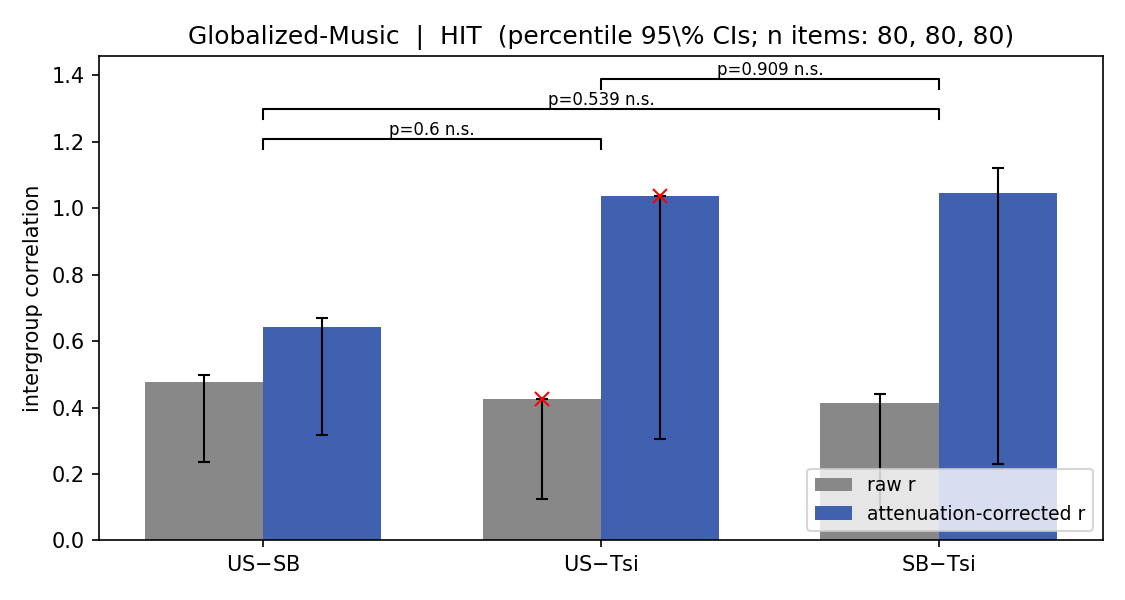
\includegraphics[width=0.85\textwidth]{figures/bar_Globalized-Music_hit.png}
\end{center}

\subsubsection*{False alarms}

\subsection*{Pairwise intergroup correlations (percentile 95\% CIs)}
\begin{center}
\begin{tabular}{lcccc}
\toprule
Pair & $\hat r$ (raw) & 95\% CI & $\hat r^*$ (corrected) & 95\% CI \\
\midrule
US$-$SB & +0.628 & [+0.415, +0.644] & +0.784 & [+0.518, +0.805] \\
US$-$Tsi & +0.245 & [+0.074, +0.342] & +0.316 & [+0.095, +0.441] \\
SB$-$Tsi & +0.424 & [+0.184, +0.476] & +0.591 & [+0.256, +0.663] \\
\bottomrule
\end{tabular}
\end{center}

\subsection*{Diagnostic --- alternative CIs on corrected $\hat r^*$}
\begin{center}
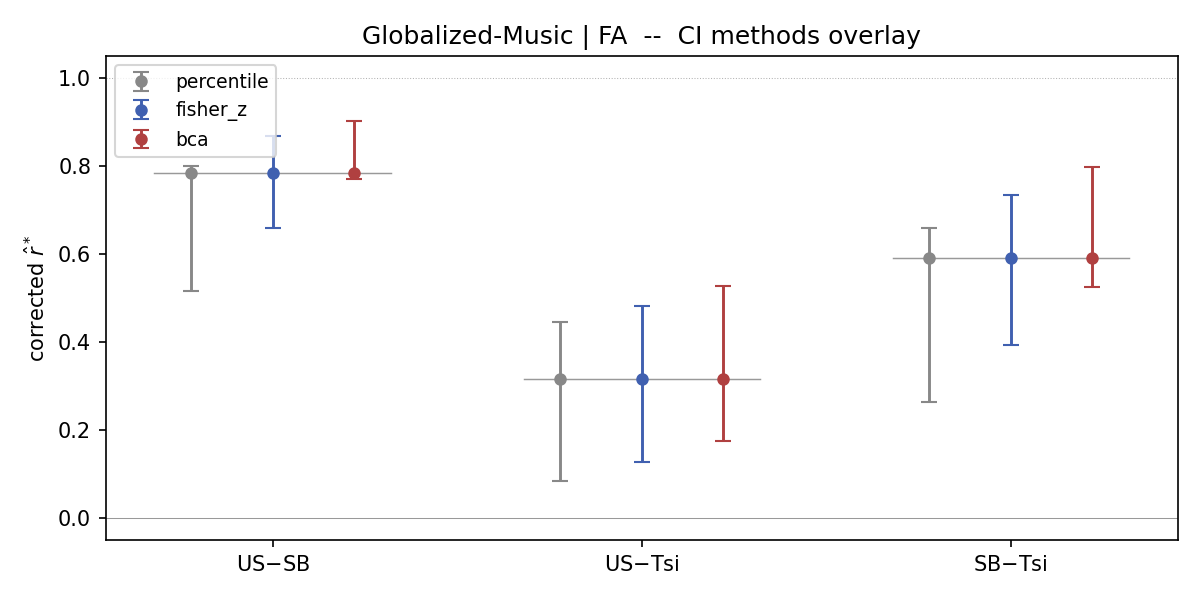
\includegraphics[width=0.85\textwidth]{figures/ci_compare_Globalized-Music_fa.png}
\end{center}

\begin{center}
\begin{tabular}{lcccc}
\toprule
Pair & $\hat r^*$ & Percentile 95\% CI & Fisher-$z$ 95\% CI & BCa 95\% CI \\
\midrule
US$-$SB & +0.784 & [+0.518, +0.805] & [+0.659, +0.867] & [+0.763, +0.898] \\
US$-$Tsi & +0.316 & [+0.095, +0.441] & [+0.134, +0.478] & [+0.179, +0.490] \\
SB$-$Tsi & +0.591 & [+0.256, +0.663] & [+0.392, +0.736] & [+0.504, +0.739] \\
\bottomrule
\end{tabular}
\end{center}

\subsection*{Stimulus-bootstrap diagnostic --- CIs on corrected $\hat r^*$ (resampling stimuli, not participants)}
\begin{center}
\begin{tabular}{lcccc}
\toprule
Pair & $\hat r^*$ & Percentile 95\% CI & Fisher-$z$ 95\% CI & BCa 95\% CI \\
\midrule
US$-$SB & +0.784 & [+0.579, +0.950] & [+0.200, +0.957] & [+0.542, +0.935] \\
US$-$Tsi & +0.316 & [+0.022, +0.587] & [+0.003, +0.573] & [+0.022, +0.586] \\
SB$-$Tsi & +0.591 & [+0.288, +0.846] & [+0.115, +0.846] & [+0.282, +0.839] \\
\bottomrule
\end{tabular}
\end{center}

\subsection*{Paired-bootstrap comparison}
\begin{center}
\begin{tabular}{lcccc}
\toprule
Comparison & Observed diff & 95\% CI (diff) & $p$ (recentered) & $p$ (straddle) \\
\midrule
US-SB vs US-Tsi & +0.383 & [+0.153, +0.493] & $<$0.001 & $<$0.001 \\
US-SB vs SB-Tsi & +0.204 & [+0.008, +0.384] & 0.031 & 0.040 \\
US-Tsi vs SB-Tsi & -0.179 & [-0.281, +0.028] & 0.025 & 0.106 \\
\bottomrule
\end{tabular}
\end{center}

\begin{center}
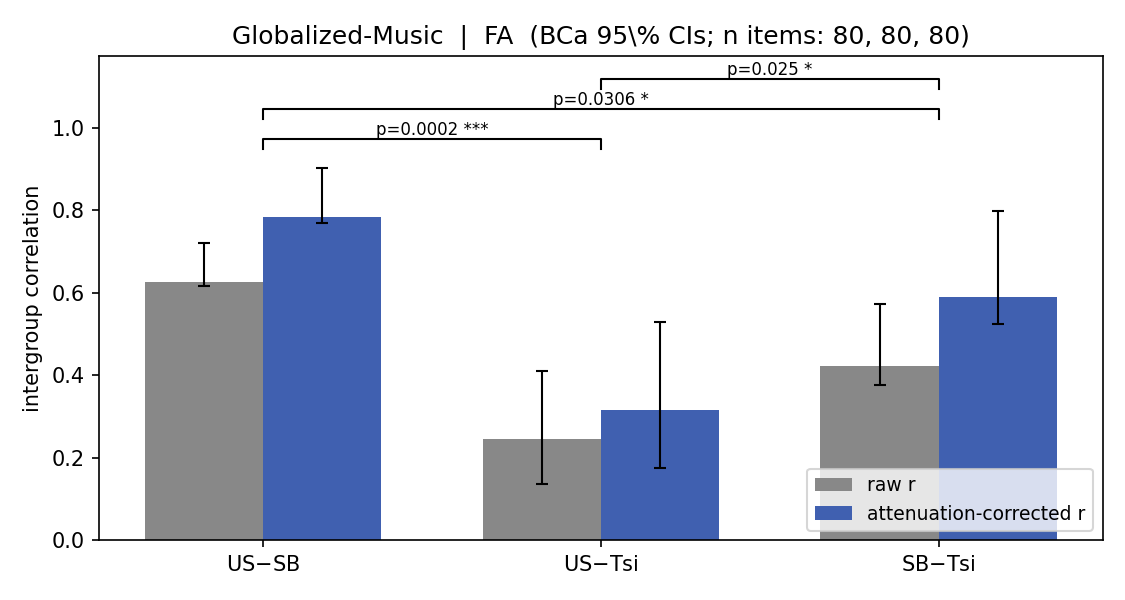
\includegraphics[width=0.85\textwidth]{figures/bar_Globalized-Music_fa.png}
\end{center}

\clearpage

\section*{Industrial-Nature}

\subsubsection*{Hits}

\subsection*{Pairwise intergroup correlations (percentile 95\% CIs)}
\begin{center}
\begin{tabular}{lcccc}
\toprule
Pair & $\hat r$ (raw) & 95\% CI & $\hat r^*$ (corrected) & 95\% CI \\
\midrule
US$-$SB & +0.623 & [+0.369, +0.607] & +0.838 & [+0.497, +0.816] \\
US$-$Tsi & +0.570 & [+0.305, +0.569] & +0.766 & [+0.410, +0.765] \\
SB$-$Tsi & +0.722 & [+0.428, +0.663] & +1.022 & [+0.605, +0.938] \\
\bottomrule
\end{tabular}
\end{center}

\subsection*{Diagnostic --- alternative CIs on corrected $\hat r^*$}
\begin{center}
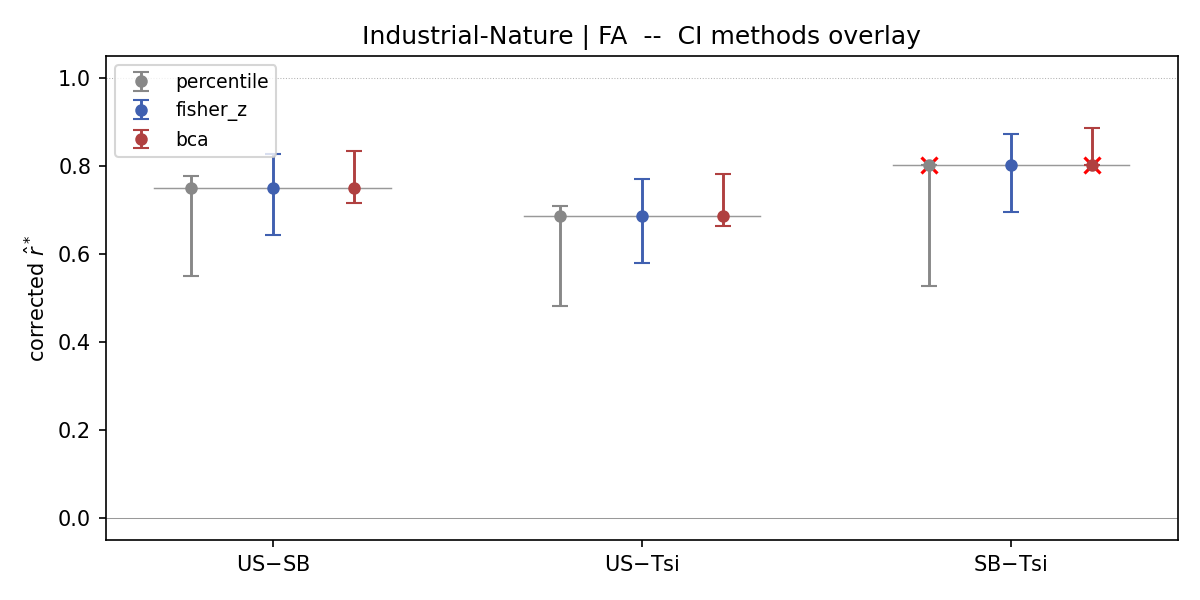
\includegraphics[width=0.85\textwidth]{figures/ci_compare_Industrial-Nature_fa.png}
\end{center}

\begin{center}
\begin{tabular}{lcccc}
\toprule
Pair & $\hat r^*$ & Percentile 95\% CI & Fisher-$z$ 95\% CI & BCa 95\% CI \\
\midrule
US$-$SB & +0.838 & [+0.497, +0.816] & [+0.725, +0.907] & [+0.856, +0.902] \\
US$-$Tsi & +0.766 & [+0.410, +0.765] & [+0.623, +0.860] & [+0.769, +0.877] \\
SB$-$Tsi & +1.022 & [+0.605, +0.938] & [+1.000, +1.000] & [+1.039, +1.039] \\
\bottomrule
\end{tabular}
\end{center}

\subsection*{Stimulus-bootstrap diagnostic --- CIs on corrected $\hat r^*$ (resampling stimuli, not participants)}
\begin{center}
\begin{tabular}{lcccc}
\toprule
Pair & $\hat r^*$ & Percentile 95\% CI & Fisher-$z$ 95\% CI & BCa 95\% CI \\
\midrule
US$-$SB & +0.838 & [+0.636, +0.993] & [-0.486, +0.995] & [+0.638, +0.994] \\
US$-$Tsi & +0.766 & [+0.563, +0.920] & [+0.356, +0.929] & [+0.568, +0.922] \\
SB$-$Tsi & +1.022 & [+0.851, +1.142] & [+0.972, +1.000] & [+0.846, +1.141] \\
\bottomrule
\end{tabular}
\end{center}

\subsection*{Paired-bootstrap comparison}
\begin{center}
\begin{tabular}{lcccc}
\toprule
Comparison & Observed diff & 95\% CI (diff) & $p$ (recentered) & $p$ (straddle) \\
\midrule
US-SB vs US-Tsi & +0.053 & [-0.098, +0.211] & 0.492 & 0.483 \\
US-SB vs SB-Tsi & -0.099 & [-0.208, +0.099] & 0.210 & 0.482 \\
US-Tsi vs SB-Tsi & -0.152 & [-0.261, +0.043] & 0.049 & 0.162 \\
\bottomrule
\end{tabular}
\end{center}

\begin{center}
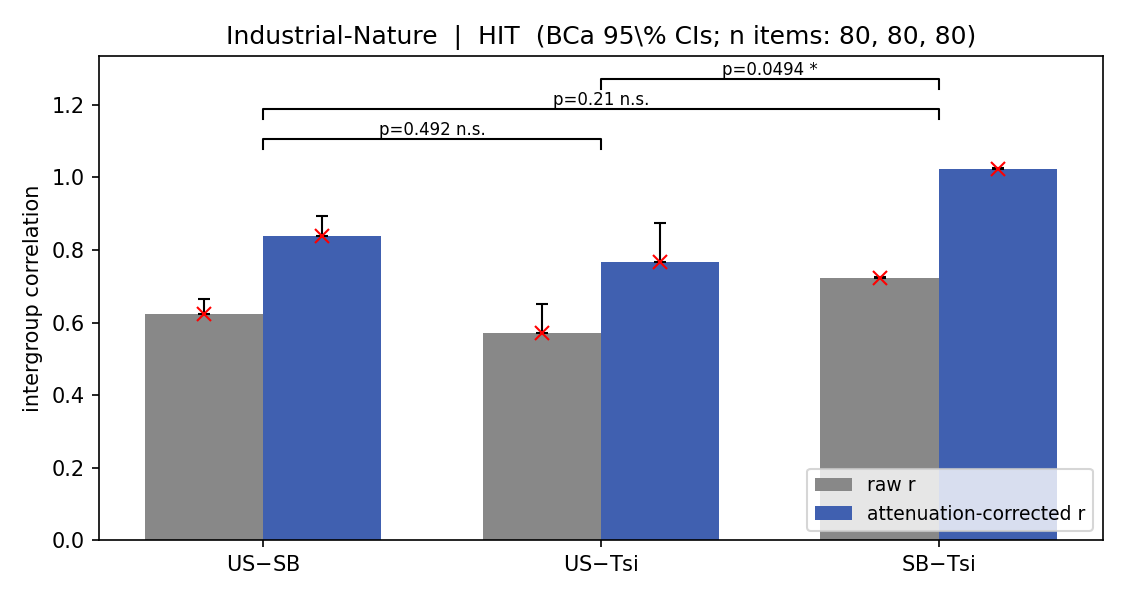
\includegraphics[width=0.85\textwidth]{figures/bar_Industrial-Nature_hit.png}
\end{center}

\subsubsection*{False alarms}

\subsection*{Pairwise intergroup correlations (percentile 95\% CIs)}
\begin{center}
\begin{tabular}{lcccc}
\toprule
Pair & $\hat r$ (raw) & 95\% CI & $\hat r^*$ (corrected) & 95\% CI \\
\midrule
US$-$SB & +0.640 & [+0.473, +0.663] & +0.750 & [+0.554, +0.776] \\
US$-$Tsi & +0.588 & [+0.409, +0.606] & +0.687 & [+0.478, +0.708] \\
SB$-$Tsi & +0.644 & [+0.428, +0.636] & +0.802 & [+0.532, +0.792] \\
\bottomrule
\end{tabular}
\end{center}

\subsection*{Diagnostic --- alternative CIs on corrected $\hat r^*$}
\begin{center}
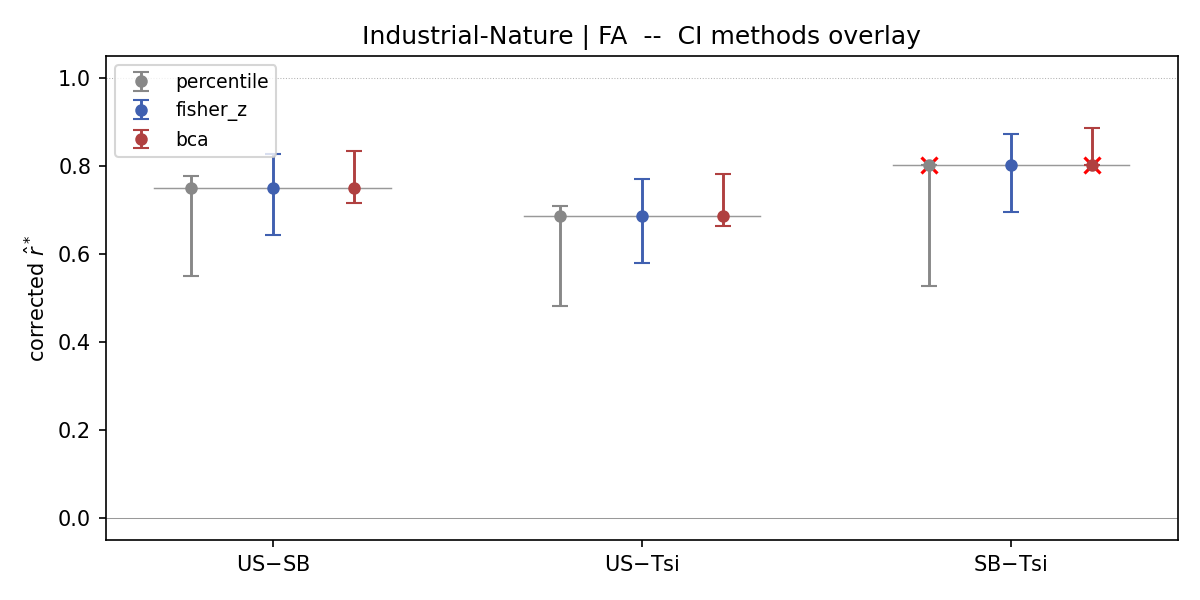
\includegraphics[width=0.85\textwidth]{figures/ci_compare_Industrial-Nature_fa.png}
\end{center}

\begin{center}
\begin{tabular}{lcccc}
\toprule
Pair & $\hat r^*$ & Percentile 95\% CI & Fisher-$z$ 95\% CI & BCa 95\% CI \\
\midrule
US$-$SB & +0.750 & [+0.554, +0.776] & [+0.645, +0.827] & [+0.723, +0.823] \\
US$-$Tsi & +0.687 & [+0.478, +0.708] & [+0.580, +0.771] & [+0.667, +0.778] \\
SB$-$Tsi & +0.802 & [+0.532, +0.792] & [+0.700, +0.872] & [+0.821, +0.877] \\
\bottomrule
\end{tabular}
\end{center}

\subsection*{Stimulus-bootstrap diagnostic --- CIs on corrected $\hat r^*$ (resampling stimuli, not participants)}
\begin{center}
\begin{tabular}{lcccc}
\toprule
Pair & $\hat r^*$ & Percentile 95\% CI & Fisher-$z$ 95\% CI & BCa 95\% CI \\
\midrule
US$-$SB & +0.750 & [+0.563, +0.893] & [+0.521, +0.878] & [+0.562, +0.893] \\
US$-$Tsi & +0.687 & [+0.485, +0.842] & [+0.459, +0.831] & [+0.488, +0.842] \\
SB$-$Tsi & +0.802 & [+0.629, +0.940] & [+0.441, +0.940] & [+0.628, +0.940] \\
\bottomrule
\end{tabular}
\end{center}

\subsection*{Paired-bootstrap comparison}
\begin{center}
\begin{tabular}{lcccc}
\toprule
Comparison & Observed diff & 95\% CI (diff) & $p$ (recentered) & $p$ (straddle) \\
\midrule
US-SB vs US-Tsi & +0.053 & [-0.069, +0.189] & 0.419 & 0.344 \\
US-SB vs SB-Tsi & -0.004 & [-0.088, +0.169] & 0.952 & 0.540 \\
US-Tsi vs SB-Tsi & -0.056 & [-0.142, +0.099] & 0.361 & 0.699 \\
\bottomrule
\end{tabular}
\end{center}

\begin{center}
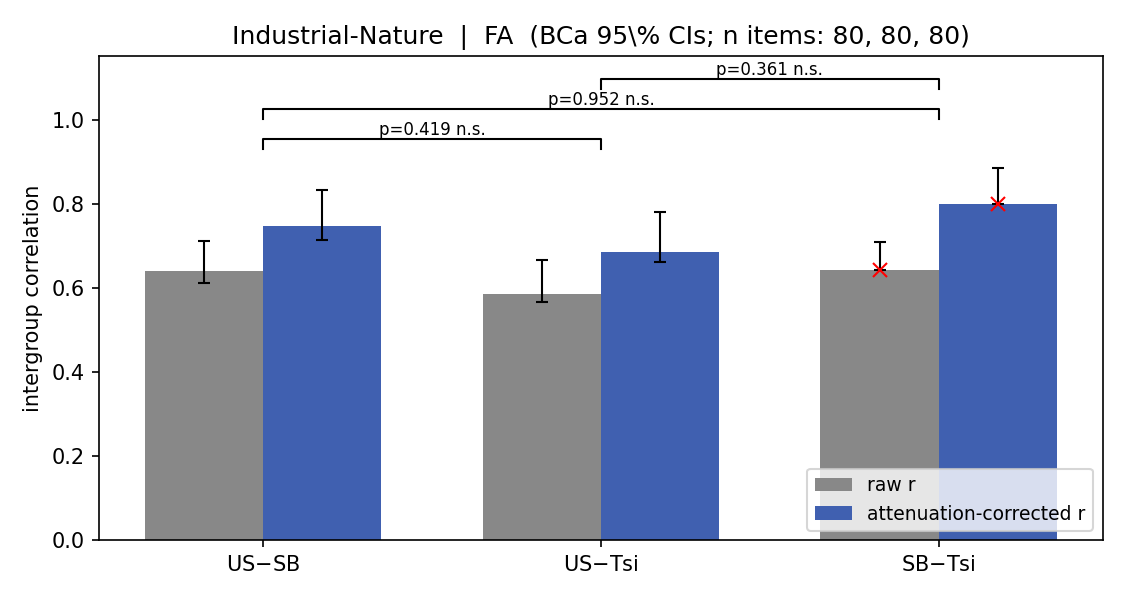
\includegraphics[width=0.85\textwidth]{figures/bar_Industrial-Nature_fa.png}
\end{center}

\clearpage

\section*{NHS}

\subsubsection*{Hits}

\subsection*{Pairwise intergroup correlations (percentile 95\% CIs)}
\begin{center}
\begin{tabular}{lcccc}
\toprule
Pair & $\hat r$ (raw) & 95\% CI & $\hat r^*$ (corrected) & 95\% CI \\
\midrule
US$-$SB & +0.491 & [+0.257, +0.515] & +0.739 & [+0.386, +0.774] \\
US$-$Tsi & +0.474 & [+0.223, +0.500] & +0.730 & [+0.344, +0.770] \\
SB$-$Tsi & +0.537 & [+0.267, +0.550] & +0.808 & [+0.402, +0.827] \\
\bottomrule
\end{tabular}
\end{center}

\subsection*{Diagnostic --- alternative CIs on corrected $\hat r^*$}
\begin{center}
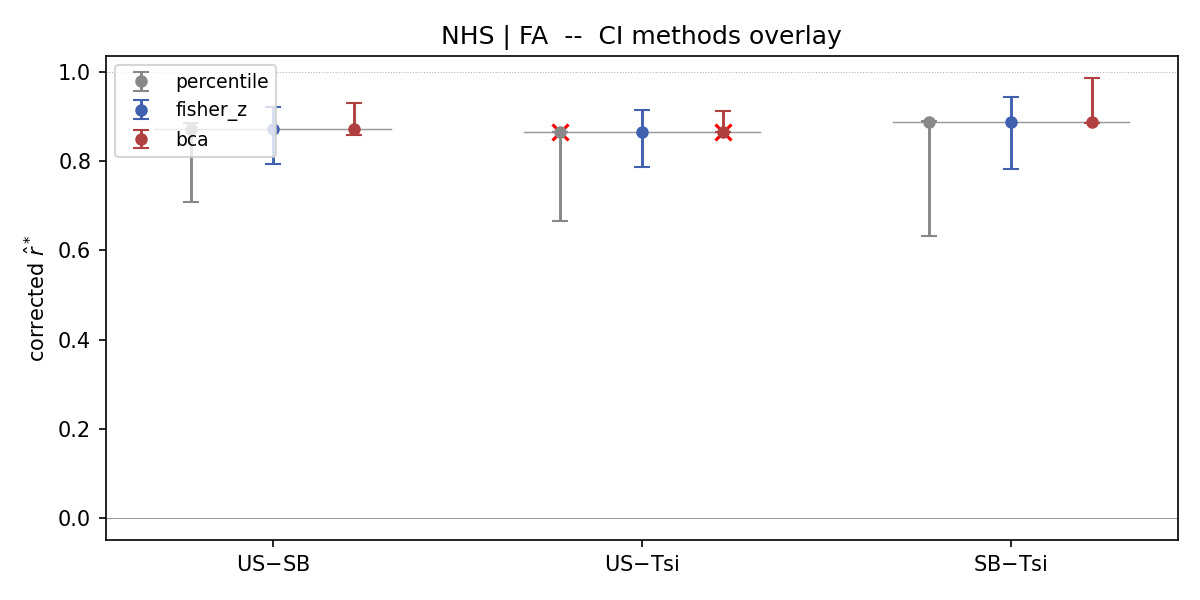
\includegraphics[width=0.85\textwidth]{figures/ci_compare_NHS_fa.png}
\end{center}

\begin{center}
\begin{tabular}{lcccc}
\toprule
Pair & $\hat r^*$ & Percentile 95\% CI & Fisher-$z$ 95\% CI & BCa 95\% CI \\
\midrule
US$-$SB & +0.739 & [+0.386, +0.774] & [+0.559, +0.853] & [+0.706, +0.937] \\
US$-$Tsi & +0.730 & [+0.344, +0.770] & [+0.535, +0.851] & [+0.690, +0.897] \\
SB$-$Tsi & +0.808 & [+0.402, +0.827] & [+0.631, +0.905] & [+0.786, +0.957] \\
\bottomrule
\end{tabular}
\end{center}

\subsection*{Stimulus-bootstrap diagnostic --- CIs on corrected $\hat r^*$ (resampling stimuli, not participants)}
\begin{center}
\begin{tabular}{lcccc}
\toprule
Pair & $\hat r^*$ & Percentile 95\% CI & Fisher-$z$ 95\% CI & BCa 95\% CI \\
\midrule
US$-$SB & +0.739 & [+0.447, +0.974] & [-0.576, +0.988] & [+0.439, +0.968] \\
US$-$Tsi & +0.730 & [+0.466, +0.961] & [-0.444, +0.981] & [+0.465, +0.958] \\
SB$-$Tsi & +0.808 & [+0.523, +1.039] & [-0.936, +0.999] & [+0.507, +1.025] \\
\bottomrule
\end{tabular}
\end{center}

\subsection*{Paired-bootstrap comparison}
\begin{center}
\begin{tabular}{lcccc}
\toprule
Comparison & Observed diff & 95\% CI (diff) & $p$ (recentered) & $p$ (straddle) \\
\midrule
US-SB vs US-Tsi & +0.017 & [-0.148, +0.182] & 0.836 & 0.819 \\
US-SB vs SB-Tsi & -0.046 & [-0.204, +0.155] & 0.626 & 0.802 \\
US-Tsi vs SB-Tsi & -0.063 & [-0.223, +0.132] & 0.486 & 0.630 \\
\bottomrule
\end{tabular}
\end{center}

\begin{center}
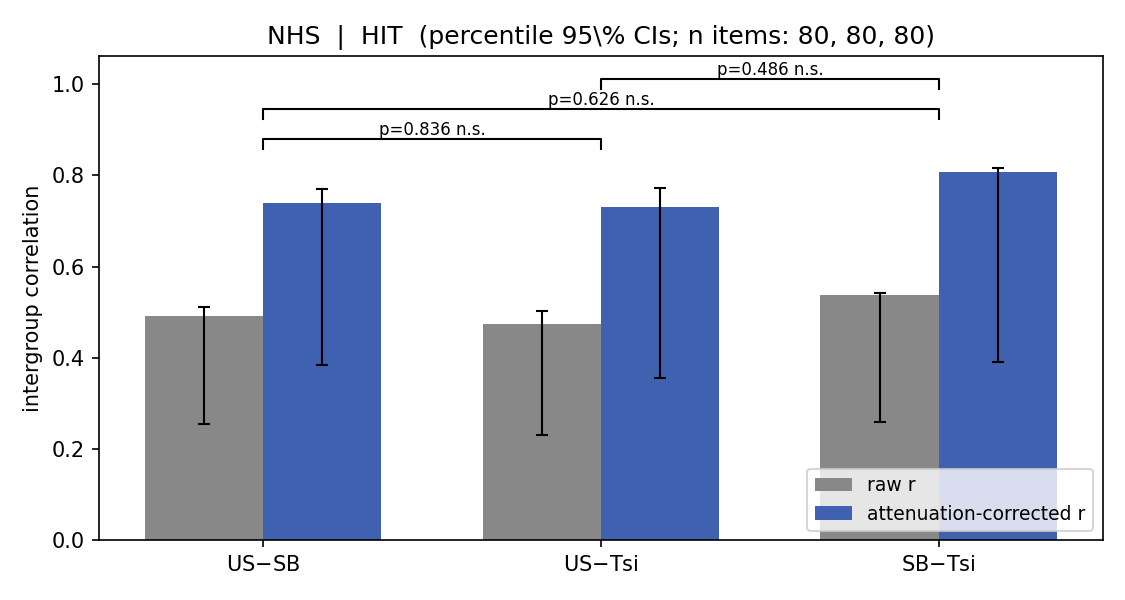
\includegraphics[width=0.85\textwidth]{figures/bar_NHS_hit.png}
\end{center}

\subsubsection*{False alarms}

\subsection*{Pairwise intergroup correlations (percentile 95\% CIs)}
\begin{center}
\begin{tabular}{lcccc}
\toprule
Pair & $\hat r$ (raw) & 95\% CI & $\hat r^*$ (corrected) & 95\% CI \\
\midrule
US$-$SB & +0.768 & [+0.620, +0.780] & +0.872 & [+0.704, +0.886] \\
US$-$Tsi & +0.753 & [+0.577, +0.750] & +0.864 & [+0.662, +0.860] \\
SB$-$Tsi & +0.748 & [+0.531, +0.756] & +0.887 & [+0.630, +0.897] \\
\bottomrule
\end{tabular}
\end{center}

\subsection*{Diagnostic --- alternative CIs on corrected $\hat r^*$}
\begin{center}
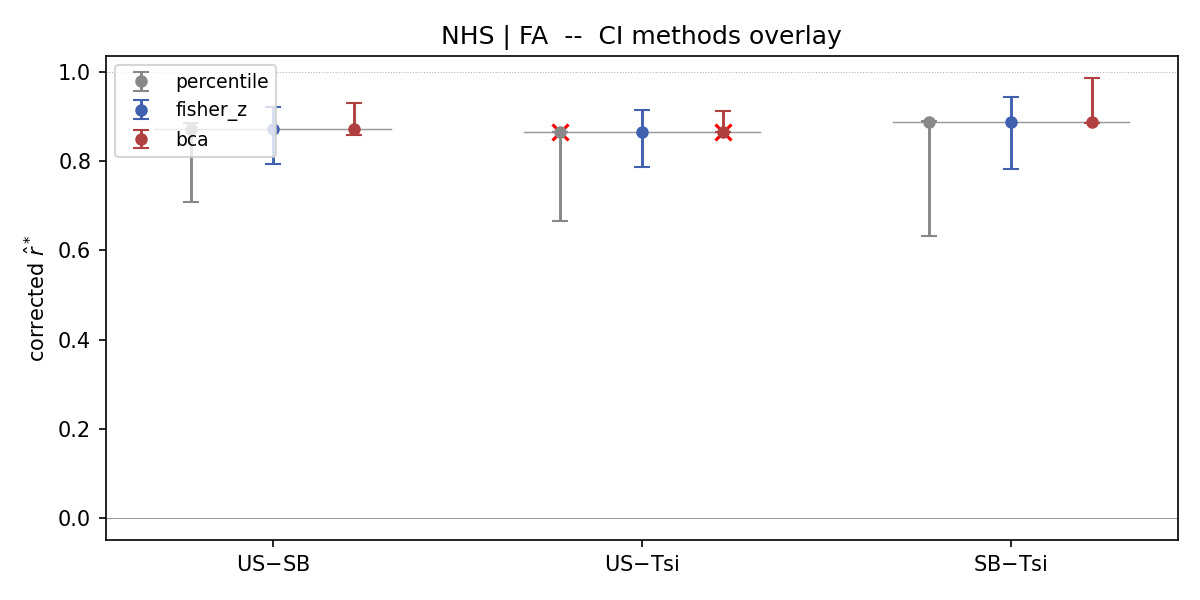
\includegraphics[width=0.85\textwidth]{figures/ci_compare_NHS_fa.png}
\end{center}

\begin{center}
\begin{tabular}{lcccc}
\toprule
Pair & $\hat r^*$ & Percentile 95\% CI & Fisher-$z$ 95\% CI & BCa 95\% CI \\
\midrule
US$-$SB & +0.872 & [+0.704, +0.886] & [+0.792, +0.922] & [+0.858, +0.939] \\
US$-$Tsi & +0.864 & [+0.662, +0.860] & [+0.785, +0.916] & [+0.866, +0.908] \\
SB$-$Tsi & +0.887 & [+0.630, +0.897] & [+0.785, +0.942] & [+0.882, +0.966] \\
\bottomrule
\end{tabular}
\end{center}

\subsection*{Stimulus-bootstrap diagnostic --- CIs on corrected $\hat r^*$ (resampling stimuli, not participants)}
\begin{center}
\begin{tabular}{lcccc}
\toprule
Pair & $\hat r^*$ & Percentile 95\% CI & Fisher-$z$ 95\% CI & BCa 95\% CI \\
\midrule
US$-$SB & +0.872 & [+0.711, +0.974] & [+0.197, +0.986] & [+0.698, +0.972] \\
US$-$Tsi & +0.864 & [+0.724, +0.960] & [+0.655, +0.950] & [+0.724, +0.962] \\
SB$-$Tsi & +0.887 & [+0.711, +1.006] & [-0.616, +0.998] & [+0.706, +1.005] \\
\bottomrule
\end{tabular}
\end{center}

\subsection*{Paired-bootstrap comparison}
\begin{center}
\begin{tabular}{lcccc}
\toprule
Comparison & Observed diff & 95\% CI (diff) & $p$ (recentered) & $p$ (straddle) \\
\midrule
US-SB vs US-Tsi & +0.015 & [-0.080, +0.149] & 0.783 & 0.531 \\
US-SB vs SB-Tsi & +0.020 & [-0.053, +0.165] & 0.716 & 0.350 \\
US-Tsi vs SB-Tsi & +0.005 & [-0.098, +0.138] & 0.926 & 0.757 \\
\bottomrule
\end{tabular}
\end{center}

\begin{center}
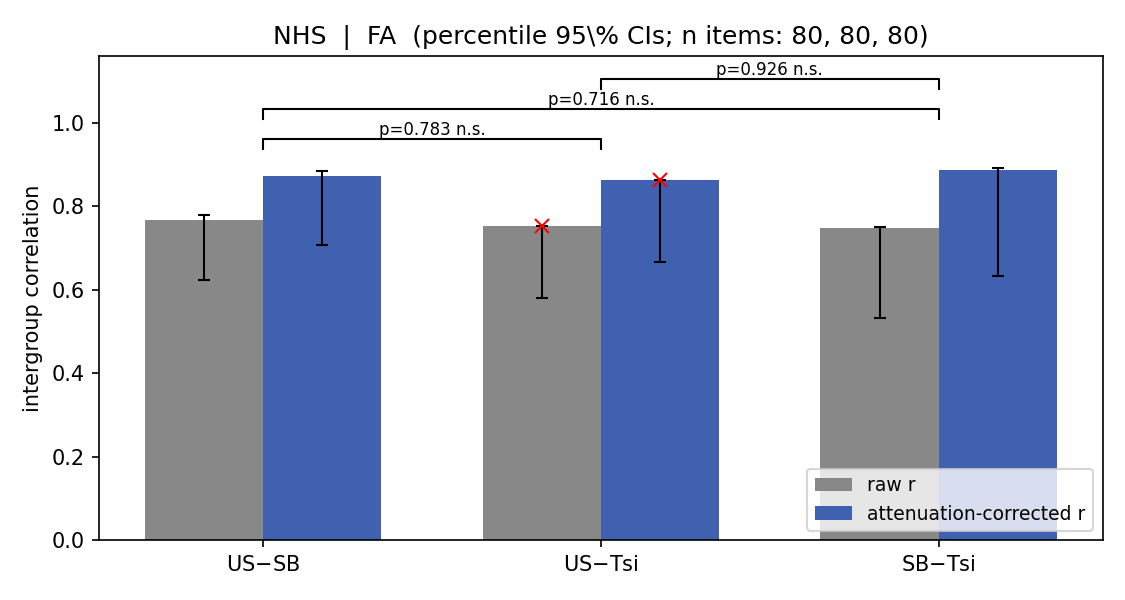
\includegraphics[width=0.85\textwidth]{figures/bar_NHS_fa.png}
\end{center}

\clearpage

\section*{Methods note}
All correlations are Spearman. Within-group reliabilities are split-half (Spearman--Brown corrected) computed by participant split. Attenuation correction applied as $\hat r^* = \hat r / \sqrt{\hat\rho^{\mathrm{SB}}_A \hat\rho^{\mathrm{SB}}_B}$; \emph{not} clamped to $[-1, 1]$ (when within-group reliabilities are small relative to the raw correlation, $\hat r^*$ can legitimately exceed 1 --- this is a property of the formula and a substantive observation about within-group noise, not a numerical failure). Bootstrap CIs computed three ways from the same resampled distribution: \textbf{percentile} (the $[\mathrm{P}_{2.5}, \mathrm{P}_{97.5}]$ quantiles), \textbf{Fisher-$z$ back-transformed} (normal-approx CI on the $z$-scale, using bootstrap $z$-space SD, centered on $\mathrm{atanh}(\hat r)$), and \textbf{BCa} (bias-corrected and accelerated with jackknife). The headline is percentile; BCa is shown in the diagnostic table. We chose percentile as the headline after observing that BCa misfires in cells with low within-group reliability (Tsimane' Globalized-Music) --- there the bias correction $\hat z_0$ becomes extreme and the corrected interval excludes the sample point estimate. Percentile is conservative under skew (wider than warranted) but doesn't break in that pathological way. Paired-bootstrap comparisons share the resample of any group that appears in both correlations under test; $p$-values are reported under two definitions, recentered-null (recommended) and straddle-zero (legacy).

\clearpage

\section*{Validation: BCa cross-check against \texttt{scipy.stats.bootstrap}}
On a vanilla synthetic case (paired bivariate-normal data, no NaNs, no coverage filter, no attenuation correction), our BCa implementation should match \texttt{scipy.stats.bootstrap(method=`BCa')}. The bootstrap distribution and the jackknife pseudo-values are constructed identically by both; the only thing being tested here is that our BCa formula matches the reference. Three known-truth cases below.

\begin{center}
\begin{tabular}{ccccccc}
\toprule
$\rho_{\text{true}}$ & $n$ & sample $\hat r$ & scipy BCa CI & our BCa CI & $\Delta$ lo & $\Delta$ hi \\
\midrule
0.30 & 80 & +0.323 & [+0.125, +0.496] & [+0.128, +0.515] & +0.0029 & +0.0188 \\
0.60 & 80 & +0.601 & [+0.426, +0.728] & [+0.440, +0.729] & +0.0143 & +0.0010 \\
0.80 & 50 & +0.850 & [+0.701, +0.925] & [+0.702, +0.925] & +0.0005 & +0.0001 \\
\bottomrule
\end{tabular}
\end{center}

\textbf{Reading the table.} The $\Delta$ columns are (ours $-$ scipy). They will not be exactly zero --- the two implementations use independent random streams, so the bootstrap distributions sampled are different. Agreement to within $\sim$0.02--0.05 across both endpoints is the expected outcome and indicates our formula and scipy's are computing the same quantity. Differences larger than that would suggest a bug in our BCa.

\end{document}
